\chapter{沙箱实验与结果分析}\label{chap:exp}

% 说明实验环境
% - 硬件环境
% - 软件环境
% - 使用偏好(Master Node)
% 软硬件说明
% - redis、mysql
% 基准测试
% - 开销分析
% 不同内核配置实验
% 隔离性实验
%  - 资源限制效果说明
% 调度策略实验
%  - 互斥调度
% 

\section{概述}

\section{实验环境}

实验环境有两台服务器构成,服务器硬件信息如表~\ref{tab:exp_env}所示。在CPU资源上,每台服务器上包含有两个Socket,单台总计80个物理核心,划分为4个Numa Node,同时,CPU均开启超线程,并使能Intel RDT,从而为可观测性基础设施提供末级缓存及内存带宽的监控,并为虚拟机提供按路数的末级缓存划分和固定补偿的内存带宽调控功能。在网络资源上,服务网卡支持SRIOV技术,能够为有网络性能需求的虚拟机提供硬件直通服务。

\begin{table}
    \bicaption{\quad 服务器硬件参数}{\quad Server Hardware Information}% caption
    \label{tab:exp_env}
    \footnotesize% fontsize
    \setlength{\tabcolsep}{4pt}% column separation
    \renewcommand{\arraystretch}{1.5}% row space 
    \centering
    \begin{tabular}{lc}
        \hline
        硬件资源 & 硬件信息 \\
        \hline
        CPU & Intel Xeon Gold 6148 (40 cores) * 2 \\
        Processor Core Frequency & 2.4GHz,Turbo 3.7 GHz \\
        L1 Caches & 32KB * 40,  8-way set associative, split D/I \\
        L2 Caches & 1024KB * 40, 16-way set associative \\
        L3 Caches & 28160KB, 11-way set associative \\
        Main Memory & 32GB * 8, 2666MHz DDR4 \\
        NIC & Intel Corporation Ethernet Connection X722 for 10GbE SFP+(10Gbit) \\
        \hline
    \end{tabular}
\end{table}

每台服务器的系统软件环境如表~\ref{tab:system_env}所示。在操作系统上,实验中选择使用较常见的Ubuntu22.04 LTS,Ubuntu同时也是Sched Ext优先支持的发行版,能够较方便地通过包管理工具安装预编译的Sched Ext内核。在虚拟换运行时上,Qemu采用发行版所支持的稳定版,而以轻量为目标的CloudHyeprvirsor则采用自编译的最新发布版本。

\begin{table}
    \bicaption{\quad 服务器系统环境}{\quad Server System Information}% caption
    \label{tab:system_env}
    \footnotesize% fontsize
    \setlength{\tabcolsep}{4pt}% column separation
    \renewcommand{\arraystretch}{1.5}% row space 
    \centering
    \begin{tabular}{lc}
        \hline
        软件类型 & 软件信息 \\
        \hline
        系统 & Ubuntu 22.04.3 LTS  \\
        内核 & 5.15.0-79-generic \\
        虚拟化运行时 & cloud-hypervisor v38.0-150 \\
                   & QEMU emulator version 6.2.0 \\
        其他        & libvirtd 8.0.0 \\
        \hline
    \end{tabular}
\end{table}

除系统软件之外,每台服务器还按照需要部署了其他关键服务。其中可观察基础设施按照第三章中所论述的架构进行搭建,Master节点上部署的了Prometheus与Grafana,用于进行数据采集与离线分析,Node节点上则部署的第三章中所提到的一系列Exporter,提供各个维度数据的采集能力。Master除对数据进行采集、存储、分析外,还额外部署了Harbor来对外提供容器管理服务,并承担大部分的配置文件存储。Node作为主要的实验场地,安装了Control Zone沙箱的所有相关的组件,并承担主要的服务运行。实验中对于Client-Server类型的任务,为尽可能地模拟真实环境,因此一般将Client放置在Master上。最后,实验中所涉及的关键服务都以容器镜像的形式分发并运行,因此在每个服务器上都需要安装容器运行时,而在容器运行时的选择上,对性能不敏感而对稳定性有要求的Master上使用Docker来提供容器服务,而在Node上,则使用Podman作为容器运行时,Podman相较Docker更加轻量,同时不存在Docker、Containerd等后台驻留服务,能够提供较为纯净的容器运行环境。

\section{沙箱性能实验}

启动开销计算从虚拟化运行时开始到系统引导至init过程的时间,虚拟化运行时上,选择CloudHyperviosr与Qemu进行对比,而在精简内核上,选择Alpine Virt内核、Control Zone内核,以及CloudHyeprvirsor、Firecracker的默认精简内核,其中Alpine Virt内核为社区提供给云厂商的标准虚拟机内核,启动了大部分Guest优化功能,但同时也保留了对于众多设备的支持,而以轻量为目标的CloudHyeprvirsor、Firecracker也各自提供了默认的精简内核,相较于Alpine Virt内核,去除了大量无意义的驱动,几乎只支持virtio设备,其中CloudHypervisor默认内核还额外使能了PCI子系统,以便于使用SRIOV设备,实验中为了让实验结果更加具备可比性,因此使能了Firecracker内核中的PCI配置。

\begin{figure}[!htbp]
    \centering
    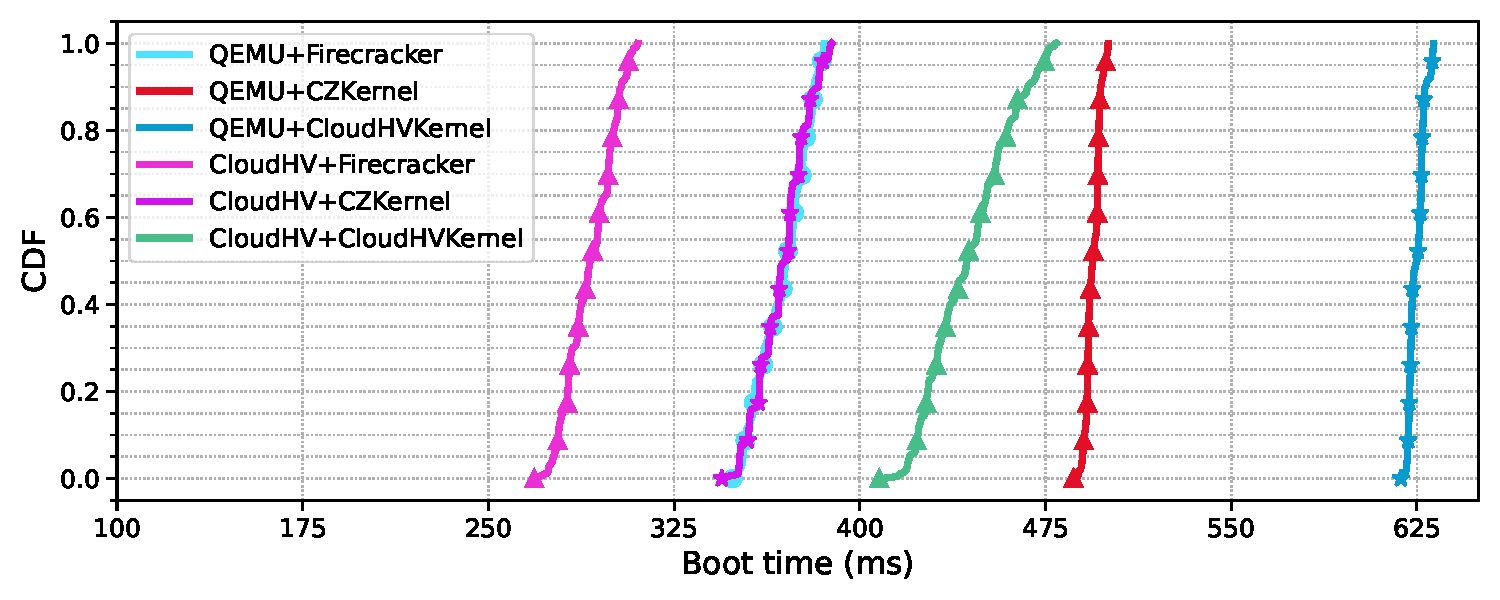
\includegraphics[width=0.8\textwidth]{boot_time_cdf}
    \bicaption{\quad Control Zone 、CloudHypervisor 及Firecracker内核的启动速度比较}{\quad The comparison of startup speed between Control Zone、CloudHypervisor and Firecracker.} 
    \label{fig:boot_time_cdf}
\end{figure}

实验结果如图~\ref{fig:avg_boot_time}所示,Control Zone内核的平均启动开销相较于Alpine Virt内核最高降低了88.8\%,对比不同的虚拟化运行时的数据发现而其中绝大部分的优化效果升来自于对内核的裁切,Control Zone内核仅支持运行容器、BPF子系统与Sched Ext调度类的最小功能,因此在启动时省去了大量非必要的工作,从而能够做到足够快速。同时还可以发现, 对于Alpine Virt内核而言,使用CloudHypervisor相较于Qemu降低28.9\%的启动时间,而观察两者的启动日志发现,虚拟化运行时所带来的提升主要来自于对于设备的裁切上,CloudHypervisor只需要针对云场景,因此相较于Qemu去除了大量的无关设备模拟,而更精简的设备一方面减少了虚拟化运行时的启动时间,另一方面,Guest内核也不必进行过多的设备探测与初始化,尤其在PCI子系统的初始化上,CloudHypervisor相较于Qemu,PCI子系统的初始化时间平均减少了83.2\%。相同的情况在其他内核上则有所不同,由于精简内核本身支持的设备驱动就十分有限,因此虚拟化运行时在这些内核的优化上主要体现在运行时启动本身上。

\begin{figure}[!htbp]
    \centering
    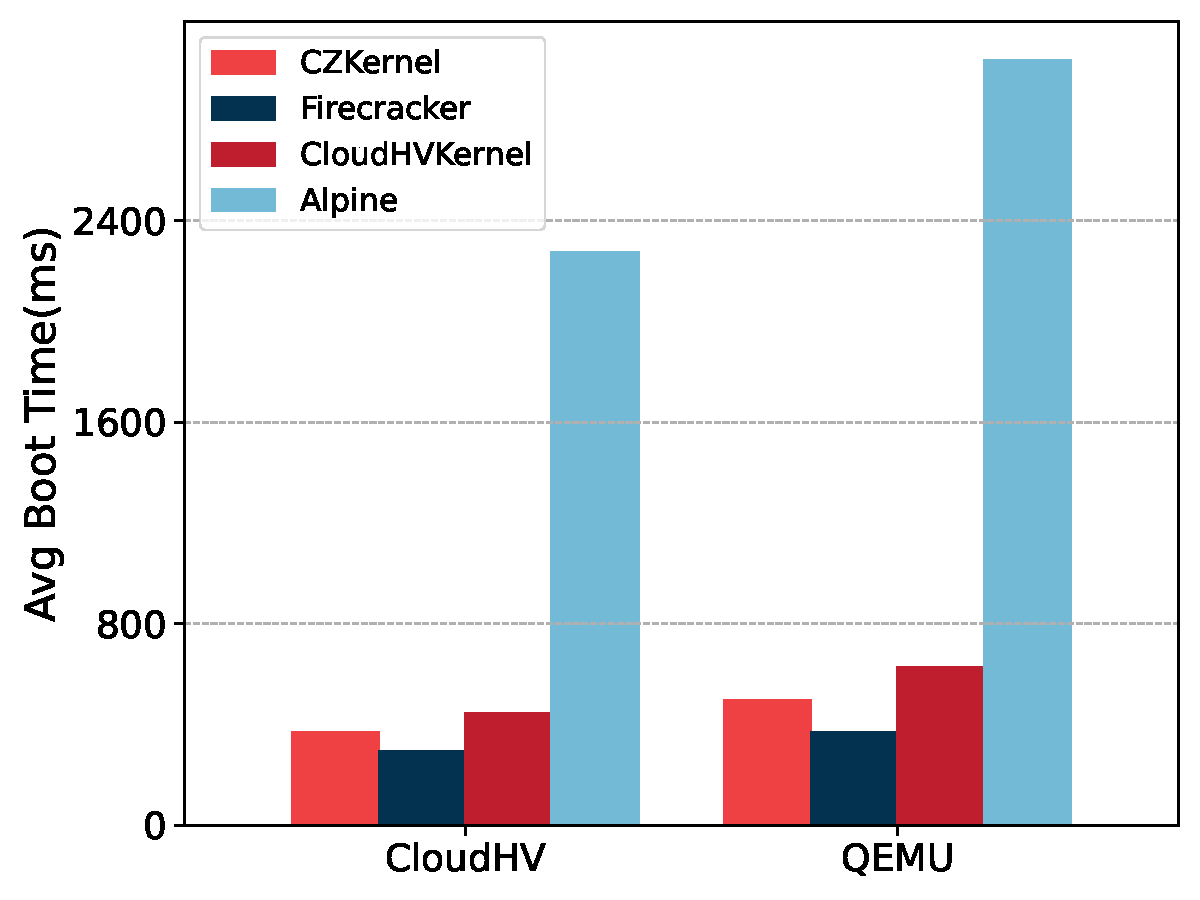
\includegraphics[width=0.7\textwidth]{avg_boot_time}
    \bicaption{\quad 启动时间为引导至运行init程序的时间,比较Firecracker(FC)、Control Zone(CZ)、Alpine(AL)内核,使用Cloud Hypervisor与Qemu}{\quad Boot time is the time it takes to boot to the init program. Compare Firecracker(FC), Control Zone(CZ), and Alpine(AL) kernels using Cloud Hypervisor and Qemu.}
    \label{fig:avg_boot_time}
\end{figure}

在精简内核的对比中,Control Zone内核也存在优势,如图~\ref{fig:boot_time_cdf}所示,使用Qemu时,Control Zone内核相较于CloudHypervisor默认内核在启动时间上减少了20.6\%,对比两者配置差异发现,CloudHypervisor所提供的精简内核虽然去掉了大部的驱动支持,但仍然保留了对嵌套虚拟化的支持而开启了虚拟化子系统,因此会产生额外的开销,而Control Zone内核所支持的容器环境所需要的支持则相对更少。但是相对于Firecra内核,Control Zone内核则在启动开销上并没有优势,即便使用Qemu虚拟化运行时,Firecracker内核也能达到接近使用CloudHypervisor的Control Zone内核的启动速度,比较配置能够发现, Firecracker内核在功能裁切上更加激进,分析两者的启动日志能够发现这开销的差异主要来自于Control Zone内核中所需要的额外功能,如Netfilter子系统等。这些功能在本设计中时必须的,同时考虑场景上的差异,Firecracker实现时希望以承担安全容器的运行时环境,虚拟机的生命周期与运行在其中的容器绑定,而在Control Zone的设计中,任务与Control Zone并非完全耦合,Control Zone更接近与对于隔离环境的声明,在任务需要运行时启动,而在任务运行完毕后仍然会保留,并提供给下一个任务使用,即Control Zone不会频繁地启动,因此这部分开销在设计中是可以接受的。

\section{可选内核性能实验}

\subsection{时钟与抢占模型}

Linux调度子系统在设计时力图覆盖足够广泛的场景,但同时也提供了一些编译配置选项,用以针对场景进行优化,这些配置选项围绕时钟与抢占模型的设置展开。

时钟与Linux调度子系统密切相关,在第二章论述中提到,时钟中断是驱动Linux抢占式调度的核心机制,中断的频率决定了调度滴答的周期,而更高的时钟中断频率意味着系统的整体响应度越好。针对时钟中断,内核主要提供了两方面的配置,如表~\ref{tab:config_hz}所示,其中最直接的就是时钟中断的频率配置,内核提供了从100、250、300到1000四种不同的中断频率配置,以满足不同的场景下对于响应度的需求,而值得注意的是,由于内核在每个时钟中断处理中进行时间记账,并将两次时钟中断所间隔的时间片累计到当前进程的记账中,然而在实际情况下两次时钟中断中间很有可能夹杂了其他任务的处理,所以更高的时钟中断频率不仅能带来响应度的提升,还能够增强任务时间记账的准确性。其次,考虑到时钟中断会引入额外的计算开销,而在一些场景中这些开销是非必要的,如当CPU进入Idle状态,此时处理时钟中断不仅没有意义,还会增加系统的开销,因此内核提供了NO\_HZ相关配置来在特定场景下屏蔽时钟中断。

\begin{table}
    \bicaption{\quad 内核时钟中断配置}{\quad Kernel Clock Interrupt Configuration}% caption
    \label{tab:config_hz}
    \footnotesize% fontsize
    \setlength{\tabcolsep}{4pt}% column separation
    \renewcommand{\arraystretch}{1.5}% row space 
    \centering
    \begin{tabular}{lc}
        \hline
        配置名称 & 描述 \\
        \hline
        HZ\_100  & 配置时钟中断频率为100  \\
        HZ\_250  & 配置时钟中断频率为250 \\
        HZ\_300  & 配置时钟中断频率为300 \\
        HZ\_1000 & 配置时钟中断频率为1000 \\
        HZ\_PERIODIC & 永远不要忽略时钟中断 \\
        NO\_HZ\_IDLE & 忽略空闲CPU上的时钟中断 \\
        NO\_HZ\_FULL & 忽略空闲CPU,以及只有一个可运行任务CPU上的时钟中断 \\
        \hline
    \end{tabular}
\end{table}

抢占指执行任务时,允许高优先级的任务打断低优先级任务的执行,从而提供更好的响应度。用户态任务的执行总是能够被打断,而内核态任务的抢占则较为复杂,为此内核提供了抢占模型的编译配置,允许用户针对不同场景进行调整,相关配置如表~\ref{tab:config_preempt}所示, 内核提供了PREEMPT\_NONE、PREEMPT\_VOLUNTARY、PREEMPT以及PREEMPT\_RT四种抢占模式,四种模式下内核的响应度逐步增强。

\begin{table}
    \bicaption{\quad 内核抢占模式配置}{\quad Kernel Preemption Configuration}% caption
    \label{tab:config_preempt}
    \footnotesize% fontsize
    \setlength{\tabcolsep}{4pt}% column separation
    \renewcommand{\arraystretch}{1.5}% row space 
    \centering
    \begin{tabular}{lc}
        \hline
        配置名称 & 描述 \\
        \hline
        PREEMPT\_NONE  & 内核代码保持执行直到主动放弃CPU  \\
        PREEMPT\_VOLUNTARY  & 开启了内核代码中的抢占位点 \\
        PREEMPT  & 提供更多的内核代码抢占位点,实现完全抢占 \\
        PREEMPT\_RT & 进一步修改内核代码的实现,如锁机制,实现实时可抢占性 \\
        \hline
    \end{tabular}
\end{table}

时钟和抢占模式的配置能够决定系统的响应度,但实际的配置需要考虑使用的场景,如更高的HZ虽然能够提升系统的整体响应度,但由于时钟中断的增多,CPU在于有限的时间片内处理实际任务的时间就会变少,同时频繁的上下文切换也破坏了程序的时间局部性,从而影响到系统的整体吞吐。通常而言,较高的HZ与激进的抢占模式有利于降低延时,而较低的HZ与保守的抢占模式有利于系统的整体吞吐。对此Control Zone提供了两种预编译的内核,用于处理响应度优先与吞吐量优先两种场景。

\subsection{响应度优先}

% redis \ keydb

Control Zone响应度优先配置使用HZ\_1000配置时钟中断,并开启PREEMPT抢占模式,并选取redis、keydb两种LC应用进行实验。


\subsection{吞吐量优先}

% graph500(time) \ ffmjpeg 

Control Zone吞吐量优先配置使用HZ\_100配置时钟中断,并开启PREEMPT\_NONE抢占模式,并选取graph500、ffmjpeg两种BE应用进行实验。实验结果如图~\ref{fig:avg_graph500_runtime}所示

% 使用竖bar图
\begin{figure}[!htbp]
    \centering
    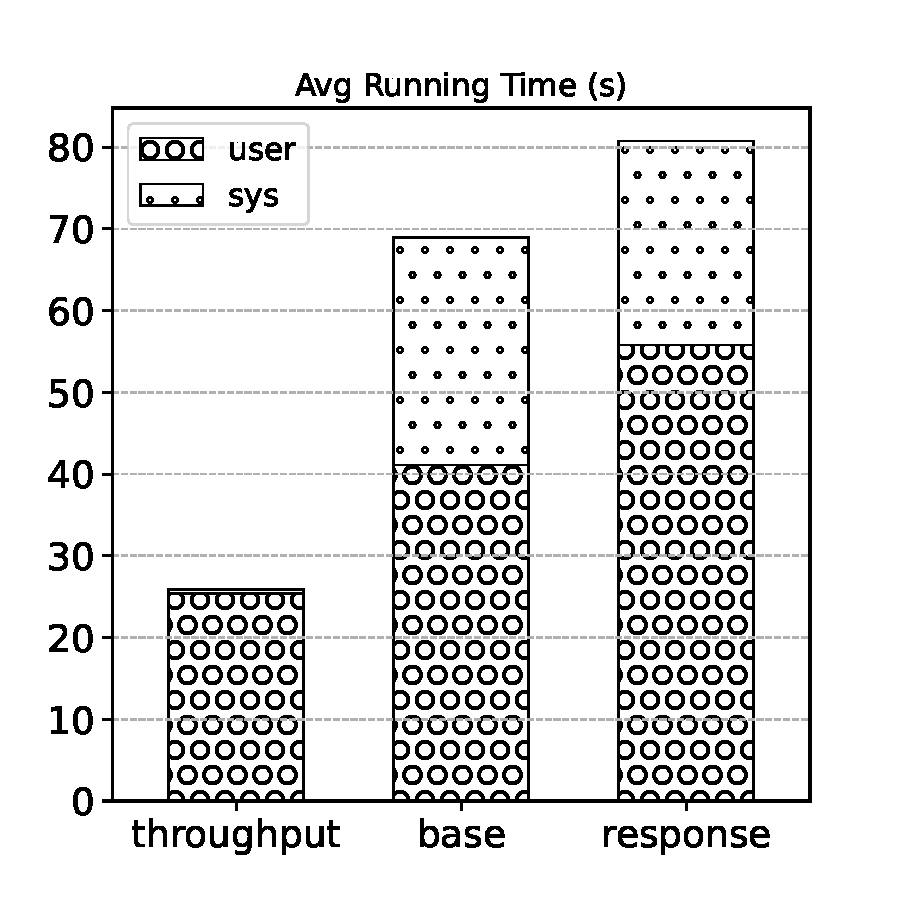
\includegraphics[width=0.8\textwidth]{avg_graph500_runtime}
    \bicaption{\quad 不同配置下的吞吐量差异}{\quad Throughput Discrepancy Across Different Configurations} 
    \label{fig:avg_graph500_runtime}
\end{figure}

\section{可选调度策略实验}

\subsection{保守调度策略}

% 增加调度策略的解释

Mysql

\begin{figure}[!htbp]
    \centering
    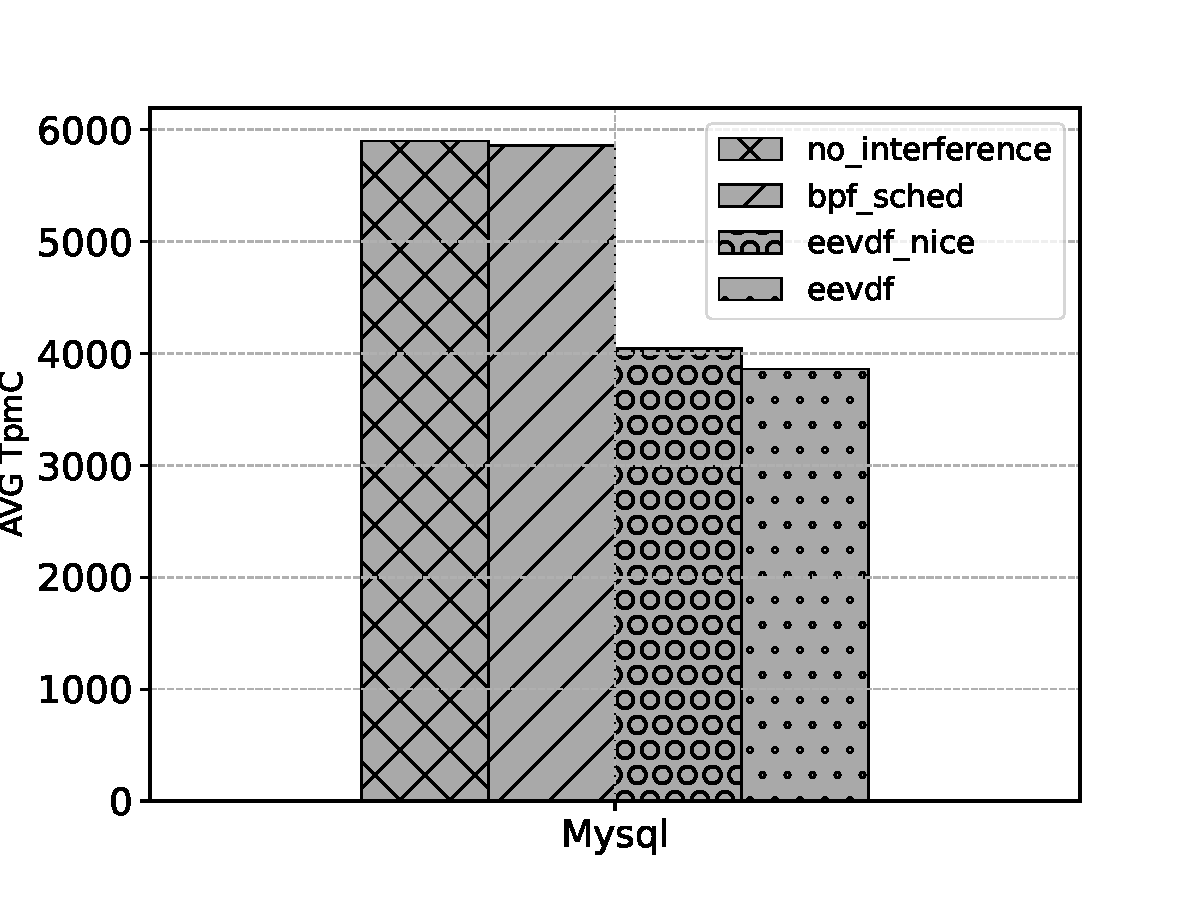
\includegraphics[width=0.8\textwidth]{mysql_perf}
    \bicaption{\quad 保守调度策略效果}{\quad Effectiveness of Conservative Scheduling Policies} 
    \label{fig:mysql_perf}
\end{figure}

% \subsection{内存资源感知策略}
% Redis

% \subsection{网络资源感知策略}

\section{本章小结}